\documentclass{article}
\usepackage[utf8]{inputenc}
\usepackage{float}

\title{ECS 145 Term Project}
\author{Gavin Grey, Jeremy Kwan, Shayan Mandegarian, Michael Nguyen}
\date{}

\usepackage{natbib}
\usepackage{graphicx}

\begin{document}

\maketitle

\section{Introduction and Goals}
Many people like to use a histogram or kernel density plot to visualize their data and the shape of the distributions. Histograms are controlled by the argument 'breaks' which changes the number of bins that are displayed in the plot. Where kernel density plots have the argument 'bw' which control the wiggliness of the curve. These arguments are called tuning parameters and are the purpose of this project. 
This assignment explores applying different tuning parameters to a dataset to generate plots of histograms or density plots. Our goal is to produce an R package that helps users explore plots based on their given parameters. We wanted to develop a solution that was not only correct, but also easy for anyone to use.
For our term project, we had to write a function of call form exploreShape(x, estMethod, tuning, twoAtATime) where x is a numeric vector, estMethod is whether we want to graph a histogram or a density graph, tuning is the number of breaks for a histogram, or the bw value of the density graph, and twoAtATime is whether we want to superimpose the previous graph onto a new graph.


\section{Graphing}

\begin{figure}[H]
\centering
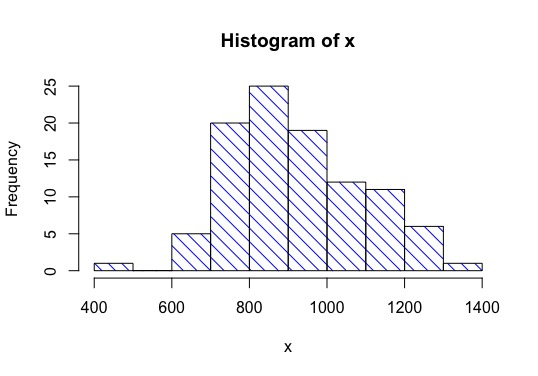
\includegraphics[scale=0.5]{Nile, 7 histogram.jpeg}
\caption{Sample output explore(Nile, 'hist', 7, T)}
\label{fig:Nile histogram 7}
\end{figure}


\begin{figure}[H]
\centering
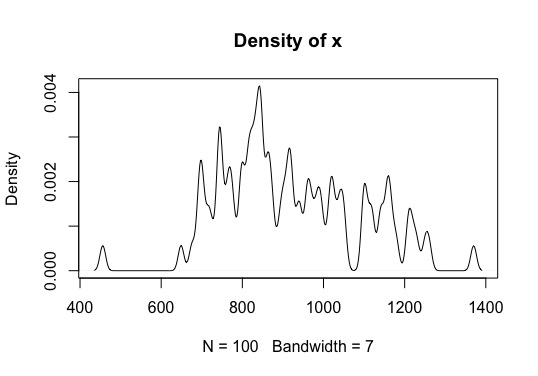
\includegraphics[scale=0.5]{Nile, 7 Tuning param.jpeg}
\caption{Sample output explore(Nile, 'density', 7, T)}
\label{fig:Nile density graph 7}
\end{figure}


\subsection{Changing Tuning Parameter}
Whenever we change the tuning parameter of the graph, if twoAtATime is initialized as true, then the previous graph is kept and superimposed onto the other graph. The previous graph is colored red to help differentiate between the graphs. To do this, we use a global variable('gmemory') that keeps track of the previous tuning parameter, so that when we graph with some new parameter, the old graph can be superimposed on top of it, and the new parameter gets stored into the global variable.

\begin{figure}[H]
\centering
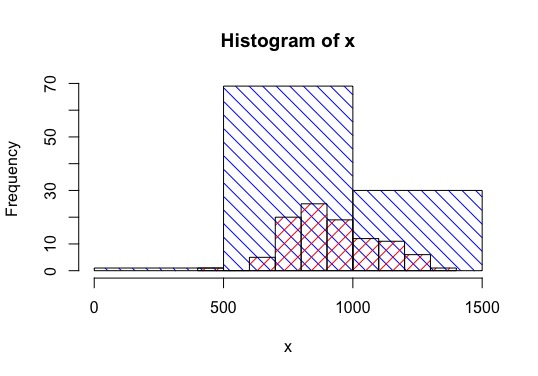
\includegraphics[scale=0.5]{Nile, 3 superimposed on 7 hist.jpeg}
\caption{Sample output explore(Nile, 'hist', 7, T), then changed tuning parameter to 3.}
\label{fig:Nile histogram 3 on 7}
\end{figure}

\begin{figure}[H]
\centering
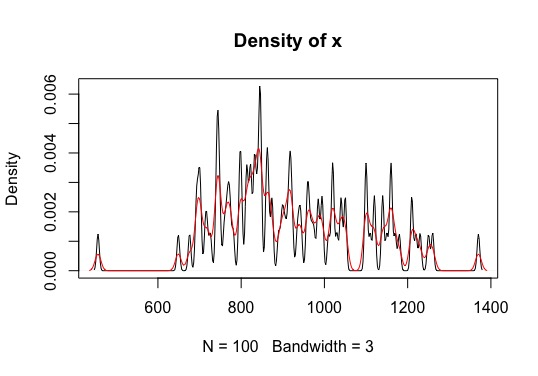
\includegraphics[scale=0.5]{Nile, 7 superimposed on 3.jpeg}
\caption{Sample output explore(Nile, 'density', 7, T) and then changed tuning parameter to 3. }
\label{fig:Nile density graph 3 on 7}
\end{figure}

\subsection{Animation}
To implement animations, we simply looped through multiple different tuning parameters, starting from 1 and stopping at 100. At each tuning parameter, the data is plotted and then the tuning parameter is incremented. This animation will not superimpose, even if the user specified to superimpose the other plots. We did not chose to use an external package to implement the animation part of this term project, but came up with a creative solution instead which uses a loop.

\subsection{Zooming In and Out}
Additionally, we included zooming functionality. This was done by first ordering the data set, then removing the first 10 and the last 10 points of data, in the case of zooming in. The amount of 'zoom in' could be adjusted through the variable 'zoomparam', which was set to 10 as the default. Then in the case of zooming out, we restore the original data set. To do this we keep the original data set stored in a global variable ('ogdata') that is set any time we pass a new data set to our function.

\begin{figure}[H]
\centering
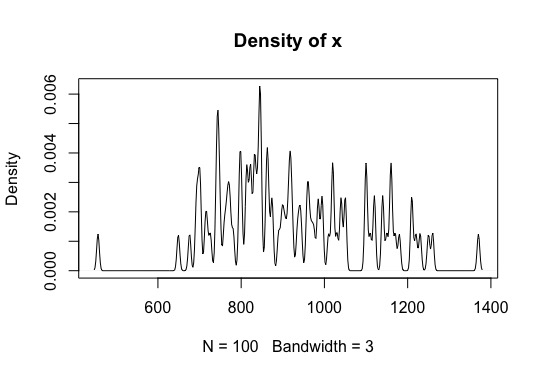
\includegraphics[scale=0.5]{Nile, 3 density before zoom.jpeg}
\caption{Sample output explore(Nile, 'density', 3, F) }
\label{fig:Nile density graph 3}
\end{figure}


\begin{figure}[H]
\centering
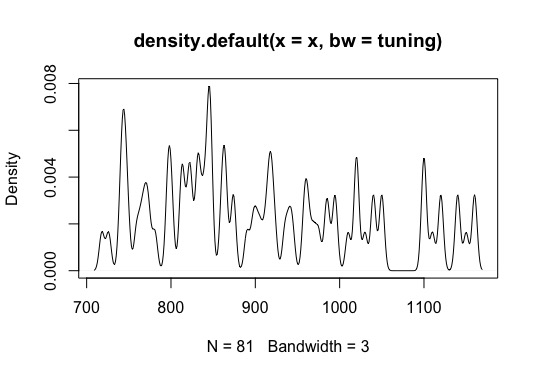
\includegraphics[scale=0.5]{Nile, 3 density after zoom in.jpeg}
\caption{Sample output explore(Nile, 'density', 3, F) zoomed in. }
\label{fig:Nile density graph 3, zoom in}
\end{figure}




\section{Individual Contributions}

\subsection{Gavin}
Gavin worked on debugging the code when errors arose, as well as brainstorming the implementation of various aspects of the code and writing the Graphing section of the report.

\subsection{Jeremy}
Initially the code was run automatically with the file, and not with a function call to exploreShape, but Jeremy put the code within the exploreShape function such that the loop and prompts went within that itself. Thus, the graphing occurred only when the user prompts it with the function exploreShape with the correct arguments. Jeremy helped with testing of the project code, and pointing out issues in output. Furthermore, Jeremy helped with outlining and organization of the report, writing the introduction as well as adding in the images of output graphs.

\subsection{Shayan}
Shayan mainly focused on improving the presentability of the project. One of the main areas of focus was making the twoAtATime
functionality work properly and easier to understand for users. At one point, we had a problem where upon first calling
exploreShape, it would still try to plot two at once using bogus data, so Shayan added code to ensure it would only plot twice
after the user gives a new tuning parameter. Also, at first was hard to view two histogram plots at once, so Shayan changed
it such that the histograms were colored with diagonal striped lines of different colors and angles. Shayan also made some
quality of life improvements like handling bad user input and allowing users to save as many tuning parameters as they want.

\subsection{Michael}
Michael started off by creating comments and empty functions to get a general idea of which direction to take the Term Project. Michael created all necessary global variables,functions and classes that would be used later in development. Michael coded the functionalities for zoom in/out, plot animations, s3 class densEst and functions. The team would go on to work on top of Michael's code to improve and adjust the project. Michael also helped in adding information to the report.

\section{Discussion}
\subsection{Assumptions and limitations}
Our project assumes that the data to be used is the Nile data set provided by the R package. We can also make it so the user would have to provide their own data set. 
The animation feature of the project only animates up to a bw / break of 100. We could possibly make it so users would be able to set their limit. 

\subsection{Scope and Style}
Throughout the coding process, we tried to provide as many informative comments about each method or variable that we used without being too verbose or ambiguous. We wrote many of the features into separate functions to keep the code clean and legible. 

\subsection{Edge Cases}

\subsection{Optimizations and Efficiency}


\subsection{Personal Reflection}
This term project has provided us with an interesting opportunity to create an R package that could be used by someone who was interested in plotting their datasets with different tuning parameters. 
This project has taught us a lot in the process of team working to building a clean and easy to use end product. 

If there was something we would do differently for next time..

\section{Conclusion}
%``I always thought something was fundamentally wrong with the universe'' %\citep{adams1995hitchhiker}

%\bibliographystyle{plain}
%\bibliography{references}

\end{document}
